\section{Mentale Modelle und Modellverständnis}
\subsection{Gestalt, Funktionalität und Fidelity}

\begin{frame}{Gestalt und Funktionalität}
\vspace{-2em}
\begin{columns}[T,onlytextwidth]
\column{.48\textwidth}
\begin{mynote}[Gestalt]
Die Gesamtheit der Formen und Strukturen, aus denen das mentale Modell einer lernenden Person besteht.
\end{mynote}
\begin{center}
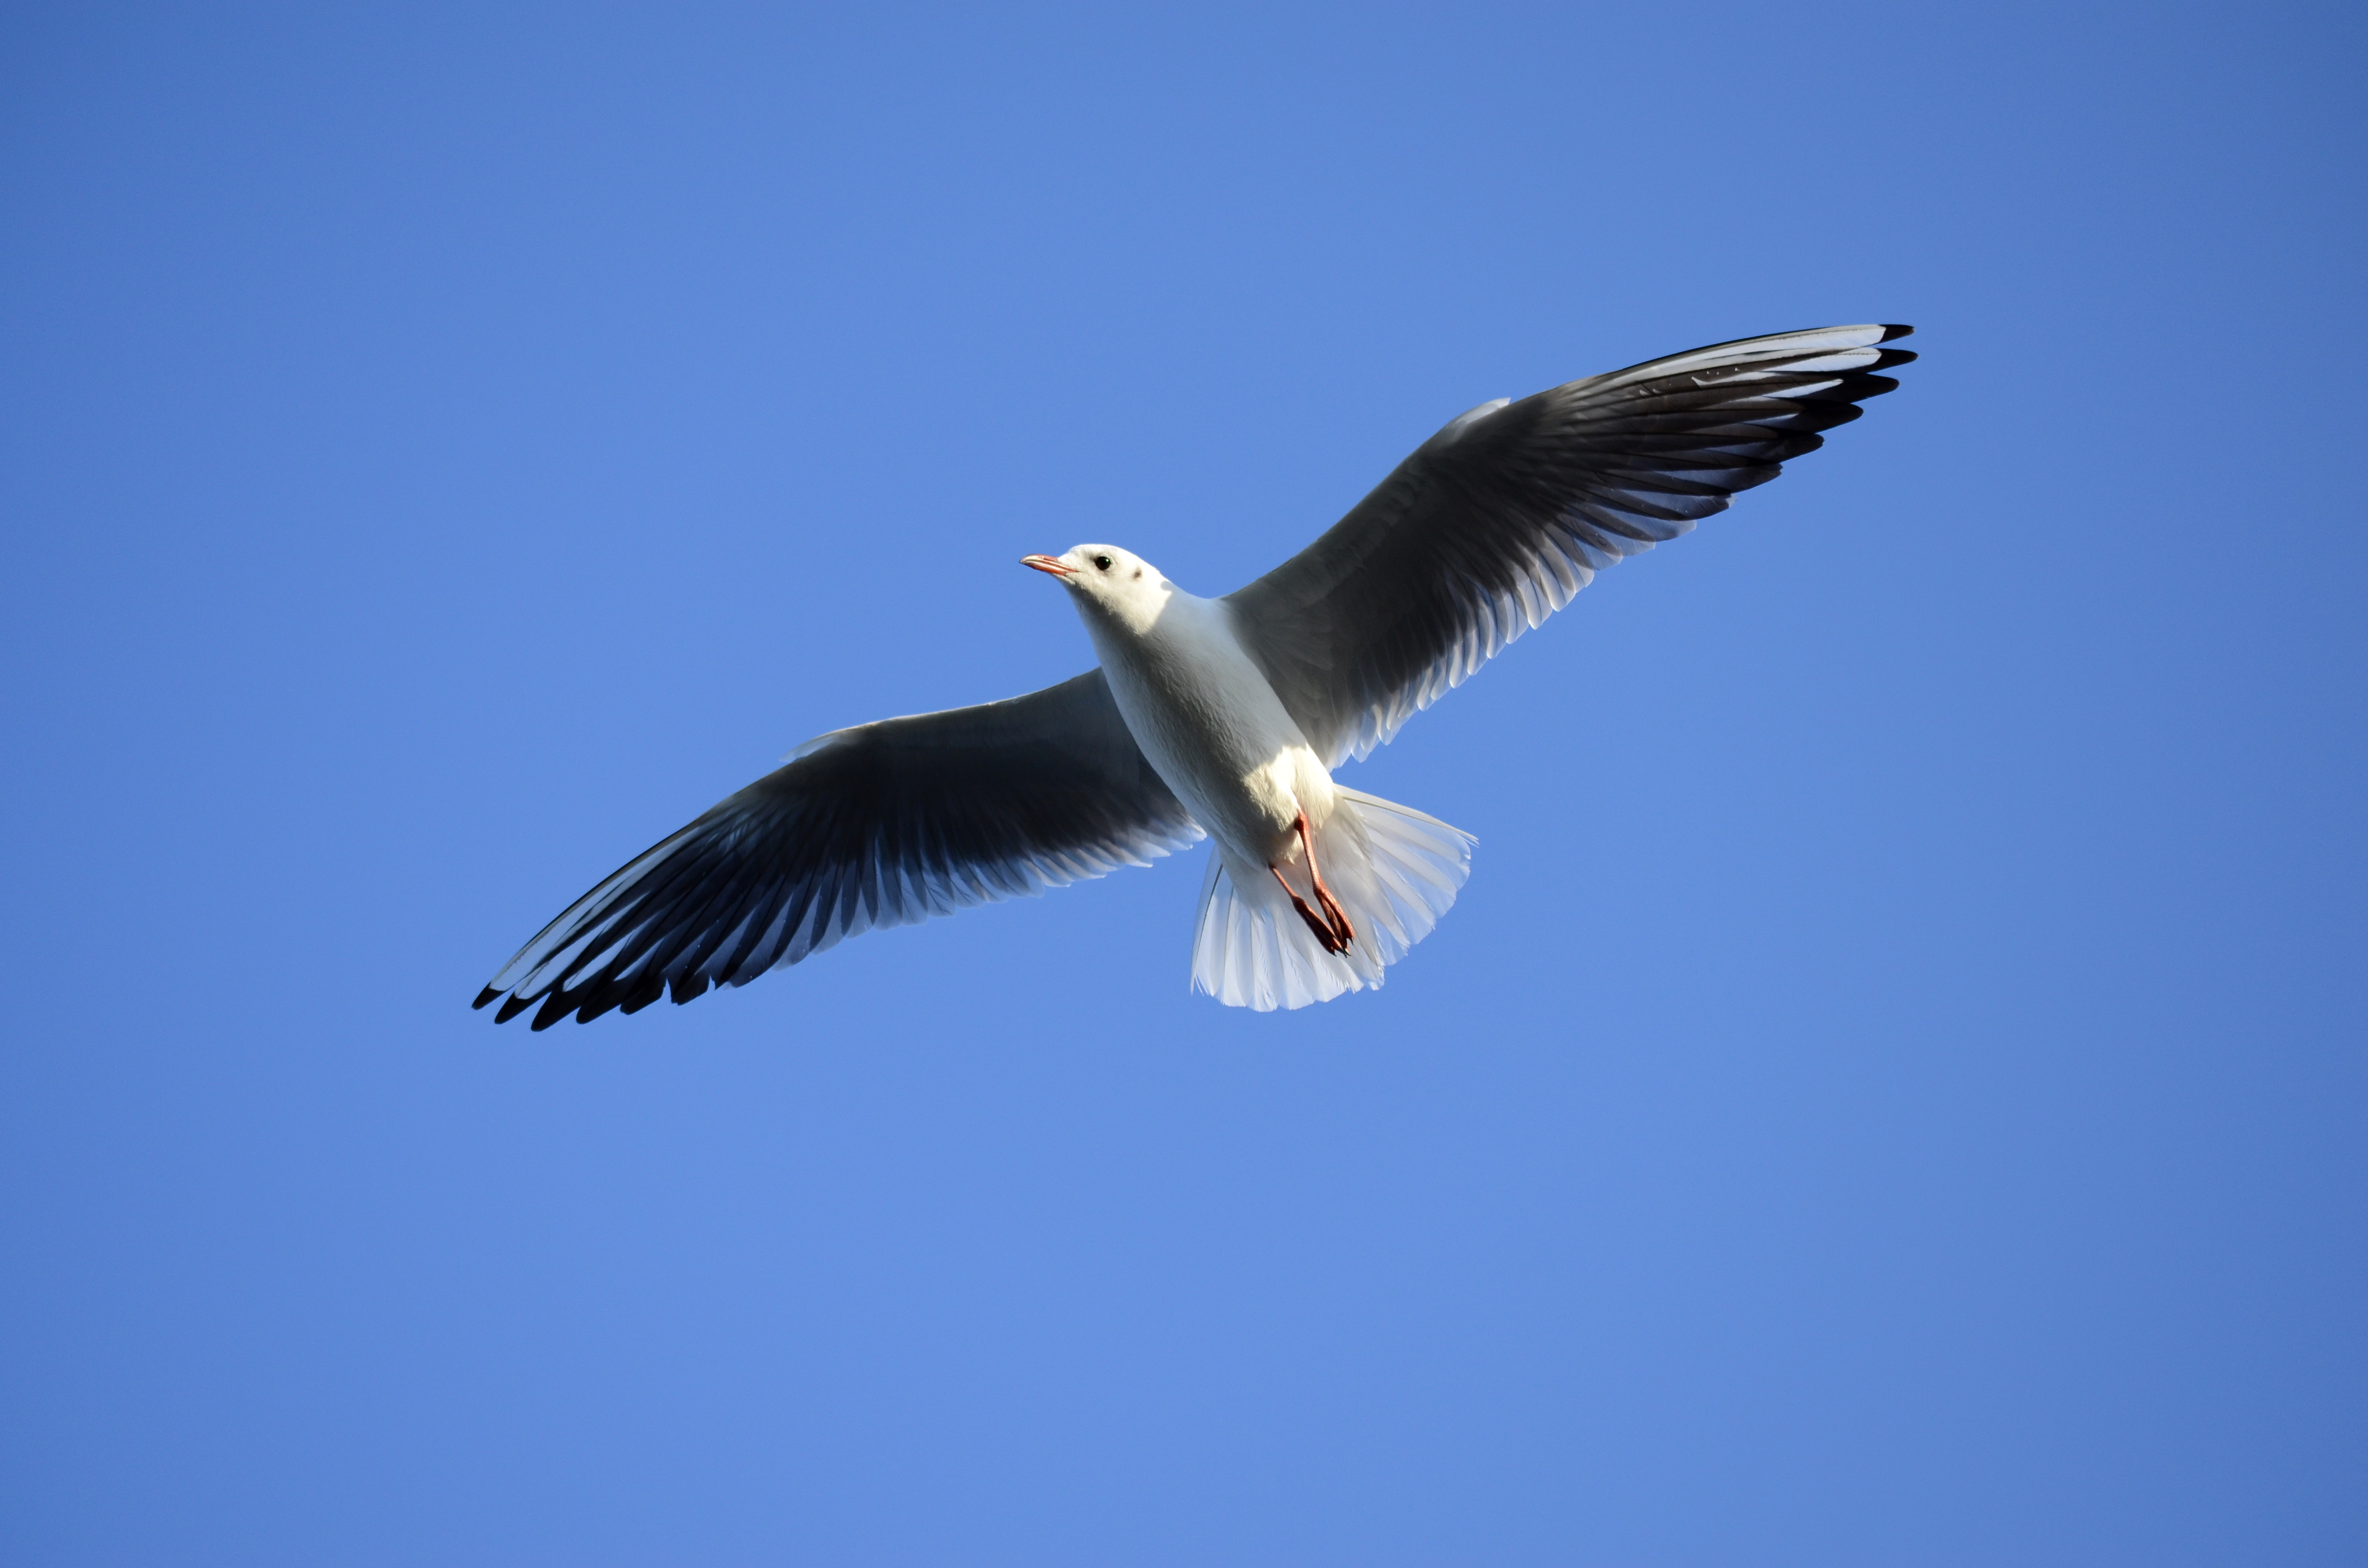
\includegraphics[width=0.7\textwidth]{images/bird.png}
\source{\citep{wiki:bird}}
\end{center}
\column{.48\textwidth}
\begin{mynote}[Funktionalität]
Die Gesamtheit der Funktionen, aus denen das mentale Modell einer lernenden Person besteht.
\end{mynote}
\begin{center}
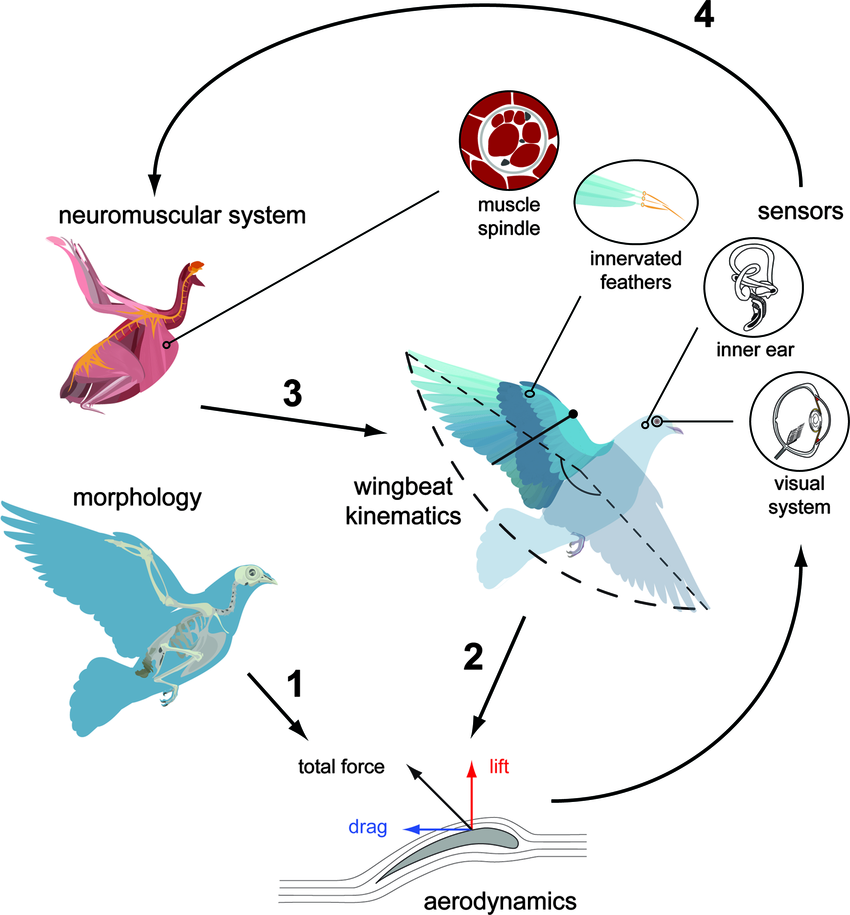
\includegraphics[width=0.5\textwidth]{images/bird_functions.png}
\source{\citep{bird_functions}}
\end{center}
\end{columns}
\slidesource{\citep{ubben2022}}
\note{Nutzen Sie das Bildpaar, um die Formen, die sich Lernende vorstellen, von den durch diese Formen kodierten Funktionen zu unterscheiden. Die Bilder müssen nicht zwingend ein realistisches einem unrealistischen Objekt gegenüberstellen.}
\end{frame}

% \begin{frame}{Mentale Modelle, wissenschaftliche Modelle und die Welt}
% \centering
% \competenciesfalse\resizebox{.94\textwidth}{!}{% Adapted from the supplied figure; coordinates compressed vertically for slides.
\begin{tikzpicture}[x=.01cm,y=-.007cm]
\draw[original] (85,686) .. controls (60,660) and (46,626) .. (46,591)
.. controls (46,504) and (122,433) .. (216,433)
.. controls (310,433) and (385,504) .. (385,591)
.. controls (385,626) and (374,659) .. (350,686)
.. controls (373,714) and (385,749) .. (385,785)
.. controls (385,872) and (310,942) .. (216,942)
.. controls (122,942) and (46,872) .. (46,785)
.. controls (46,748) and (60,713) .. (85,686);
\draw[original,densely dotted] (85,686)--(350,686);
\draw[original] (650,316) .. controls (637,295) and (630,272) .. (630,248)
.. controls (630,161) and (706,90) .. (800,90)
.. controls (894,90) and (970,161) .. (970,248)
.. controls (970,273) and (964,296) .. (952,316)
.. controls (963,338) and (969,360) .. (969,384)
.. controls (969,471) and (893,541) .. (800,541)
.. controls (706,541) and (629,471) .. (629,384)
.. controls (629,359) and (637,335) .. (650,316);
\draw[original,densely dotted] (650,316)--(952,316);
\draw[original] (1180,432) rectangle (1518,942);
\draw[original] (1180,686)--(1518,686);
\draw[relation] (412,569)--(1141,569);
\draw[relation] (412,808)--(1141,808);
\draw[relation,alignmentblue] (385,571)--(632,246);
\draw[relation,alignmentblue] (385,786)--(637,466);
\draw[relation,modellingorange] (970,246)--(1180,578);
\draw[relation,modellingorange] (950,470)--(1180,812);
\node[maintext] at (216,387) {Mentale Modelle};
\node[maintext] at (797,45) {Physikalisches Modell};
\node[maintext] at (1348,387) {Reales Phänomen};
\node[maintext] at (217,561) {Gestalt};
\node[maintext] at (217,815) {Funktionalität};
\node[maintext] at (800,204) {Ausgewählte Formen\\und Strukturen};
\node[maintext] at (800,402) {Ausgewählte\\Funktionen};
\node[maintext] at (1348,561) {Sinnliche\\Muster};
\node[maintext] at (1348,815) {Funktionen};
\node[labelbox,text=alignmentblue] at (492,390) {Strukturelles\\Alignment};
\node[labelbox,text=alignmentblue] at (504,694) {Funktionales\\Alignment};
\node[labelbox,text=modellingorange] at (1075,340) {Strukturelle\\Modellierung};
\node[labelbox,text=modellingorange] at (1075,694) {Funktionale\\Modellierung};
\node[labelbox] at (777,620) {Fidelity of Gestalt};
\node[labelbox] at (792,862) {Functional Fidelity};
\ifcompetencies
\node[badge] at (602,370) {1};
\node[badge] at (620,690) {2};
\node[badge] at (1160,240) {3};
\node[badge] at (1165,630) {4};
\node[badge] at (980,45) {5};
\node[badge] at (967,620) {6};
\node[badge] at (983,862) {6};
\draw[feedback] (1350,950) .. controls (1350,1006) and (1310,1020) .. (1230,1020)
-- (80,1020) .. controls (-62,1020) and (-65,956) .. (-65,861)
-- (-65,648) .. controls (-65,590) and (-28,590) .. (44,590);
\draw[feedback] (-65,850) .. controls (-65,793) and (-20,793) .. (43,793);
\node[labelbox,text=competencygreen] at (770,1020)
{\textbf{Testen, bewerten und revidieren}\\Gestalt und Funktionalität anhand von Evidenz anpassen};
\node[badge] at (210,1020) {7};
\fi
\end{tikzpicture}
}
% \source{Gemeinsame Arbeit von Judith Schmid, Malte Ubben, Fabian Hennig, Jonas Bley und Philipp Bitzenbauer (unveröffentlicht, 2026). Schwarz: Fidelity; Blau: Experten-Alignment; Orange: wissenschaftliche Modellierung.}
% \end{frame}

%\begin{frame}{Fidelity-Überzeugungen innerhalb des Modellverständnisses}
%\begin{tabularx}{\textwidth}{@{}P{.23\textwidth}YY@{}}
%\toprule
%& \textbf{Fidelity of Gestalt (FG)} & \textbf{Functional Fidelity (FF)}\\
%\midrule
%Überzeugung der Lernenden & Wie genau bildet mein Modell ab, wie das Phänomen aussieht? & Wie angemessen beschreibt mein Modell, wie das Phänomen funktioniert?\\
%Hohe Ausprägung & Starke Überzeugung von sensorischer oder visueller Originaltreue. & Starke Überzeugung von funktionaler Angemessenheit.\\
%Interpretation & Kann wörtliche Lesarten abstrakter Abbildungen begünstigen. & Kann die Wertschätzung von Vorhersage und Erklärung unterstützen.\\
%\bottomrule
%\end{tabularx}\par
%\keyidea{FF und FG erfassen Fidelity-Überzeugungen. FA und GA erfassen das Experten-Alignment innerhalb des Modellverständnisses.}
%\source{\citep{ubben2022}; Beispiele und Anwendung auf Polarisation für diese Studie adaptiert.}
%\end{frame}

\begin{frame}{Vier Profile von Fidelity-Überzeugungen}
\centering
\begin{tikzpicture}
\draw[-{Stealth},thick] (0,0)--(10.8,0) node[right] {FF};
\draw[-{Stealth},thick] (0,0)--(0,4.6) node[above] {FG};
\draw[gray,dashed] (5.2,0)--(5.2,4.2);
\draw[gray,dashed] (0,2.1)--(10.4,2.1);
\node[align=center,text width=4.7cm] at (2.6,3.2) {\textbf{Architektonisch}\\Hohe FG, geringe FF\\Fokus auf Erscheinungsbild};
\node[align=center,text width=4.7cm] at (7.8,3.2) {\textbf{Dual}\\Hohe FG, hohe FF\\Visueller Realismus und Funktion};
\node[align=center,text width=4.7cm] at (2.6,1) {\textbf{Unausgeprägt}\\Geringe FG, geringe FF};
\node[align=center,text width=4.7cm] at (7.8,1) {\textbf{Funktional}\\Geringe FG, hohe FF\\Funktion ohne Abbild-Annahme};
\end{tikzpicture}
\source{\citep{ubben2022,bitzenbauer2025}}
\note{FF und FG sind kontinuierliche Dimensionen. Die vier Profile beschreiben Kombinationen, keine starren Kategorien von Lernenden. Bitzenbauer und Ubben (2025) liefern konfirmatorische Evidenz im Photonen-Kontext und schlagen das Fidelities-Modell der Konzeptentwicklung vor. Ihr Entwicklungsansatz motiviert mögliche Übergänge, belegt jedoch nicht, dass dieses Polarisations-Applet sie verursacht.}
\end{frame}

\subsection{Experten-Alignment}
\begin{frame}{Fidelity und Alignment im Vergleich}
\begin{columns}[T,onlytextwidth]
\column{.47\textwidth}
\textbf{Fidelity: Haltung der Lernenden}
\begin{itemize}
\item In welcher Hinsicht halten Lernende das Modell für originalgetreu?
\item FG: Erscheinungsbild; FF: Funktion.
\end{itemize}
\column{.49\textwidth}
\textbf{Alignment: Experten-Übereinstimmung}
\begin{itemize}
\item \textbf{Strukturelles/Gestalt-Alignment (GA):} Übereinstimmung mit von Expert:innen ausgewählten Formen und Strukturen.
\item \textbf{Funktionales Alignment (FA):} Übereinstimmung mit von Expert:innen ausgewählten Funktionen.
\end{itemize}
\end{columns}
\vspace{1.5mm}
\keyidea{Erfolgreiches visuelles Schlussfolgern kann mit wörtlichen Modellüberzeugungen koexistieren.}
\source{Studie zu Polarisation und Zustandskreis: \citep{toth2024}.}
\note{GA ist die Bezeichnung der Studie für das strukturelle/Gestalt-Alignment, im theoretischen Rahmen auch StA genannt. FA bezeichnet das funktionale Alignment. Toth, Michelini und Bitzenbauer (2024) beschreiben Lernende der Sekundarstufe I, die erfolgreich mit einer Zustandskreis-Visualisierung argumentierten und zugleich gestaltbezogene Vorstellungen beibehielten. Dies stützt die Unterscheidung von Fidelity-Überzeugungen und Leistung, belegt jedoch noch nicht die Wirkung unserer Kugel bei Studierenden. Lernende können ein korrektes Kugeldiagramm reproduzieren und es dennoch als physisches Objekt rund um den Lichtstrahl auffassen.}
\end{frame}

\begin{frame}{Visualisierung und der Multimedia-Effekt}
\small
\vspace{-1.3em}
\begin{myalert}[Multimedia-Prinzip]
Die Kombination von Wörtern mit relevanten Bildern kann Lernende stärker unterstützen als Wörter allein.
\source{\citep{Mayer2005Cognitive}}
% Learners need to connect the verbal and pictorial representations with their prior knowledge.
\end{myalert}
\vspace{-0.4em}
\begin{mynote}[DeFT: Design, Funktionen, Aufgaben]
\begin{itemize}\setlength{\itemsep}{1pt}
    \item \textbf{Design:} Anzahl der Repräsentationen, Informationsverteilung, Form, Reihenfolge sowie Hervorhebung der Übersetzungen.
    \item \textbf{Funktionen (Functions):} Repräsentationen können einander \textbf{ergänzen}, Interpretationen \textbf{einschränken} und den Aufbau eines \textbf{tieferen Verständnisses} unterstützen.
    \item \textbf{Aufgaben (Tasks):} Erforderliche kognitive Anforderungen: die Repräsentationen und ihre Beziehungen verstehen sowie passend auswählen.
\end{itemize}
\vspace{-0.4em}
\source{\citep{ainsworth2006}}
\end{mynote}
%\vspace{-0.3em}
% \keyidea{The sphere may support functional reasoning,
% but connecting it with the other views also creates
% cognitive demands.}

\note{
Das Multimedia-Prinzip motiviert die Kombination verbaler und
bildhafter Informationen. Es impliziert nicht, dass das Hinzufügen weiterer
Visualisierungen das Lernen zwangsläufig verbessert.

Beide Studienbedingungen enthalten bereits multiple Repräsentationen.
Unser Vergleich untersucht daher den Beitrag einer
zusätzlichen Repräsentation, statt direkt Wörter plus Bilder
gegen Wörter allein zu testen.

Übertragen auf diese Studie kann die Kugel die Jones-Notation
und den räumlichen Wellengraphen ergänzen, indem sie Zustandsbeziehungen und
Transformationen sichtbar macht. Korrespondenzen zwischen den Ansichten können
irreführende Interpretationen einschränken. Das Verknüpfen ihrer gemeinsamen
funktionalen Beziehungen kann ein tieferes Verständnis unterstützen.

Dies sind angenommene Funktionen, keine garantierten Effekte.
Lernende müssen die Konventionen der Kugel verstehen und sie mit
den anderen Repräsentationen verknüpfen. Diese Anforderungen können auch
Schwierigkeiten oder zusätzliche kognitive Belastung (Cognitive Load) erzeugen.

Im DeFT-Rahmen bezieht sich „Tasks“ auf die von den Lernenden geforderte
kognitive Arbeit. Es impliziert keine zusätzlichen Interview-Aktivitäten.
Laut-Denken-Beobachtungen erfassen spontanes Schlussfolgern während
der bestehenden Applet-Aufgaben, ohne zusätzliche Fragen oder Impulse.
}
\end{frame}

\begin{frame}{Zwei Wirkpfade einer zusätzlichen Visualisierung}
\begin{columns}[T,onlytextwidth]
\column{.48\textwidth}
\begin{mynote}[Repräsentationale Unterstützung]
\begin{itemize}
\item Ergänzung durch verschiedene Strategien zur Problemlösung.
\item Verknüpfung von Notation, Geometrie und optischen Transformationen.
\item Unterstützung expertenkonformer Erklärungen und Vorhersagen.
\end{itemize}
\end{mynote}
\column{.48\textwidth}
\begin{mynote}[Spontane Reflexion]
\begin{itemize}
\item Begegnung mit unterschiedlichen Repräsentationen desselben Zustands.
\item Hinterfragen wörtlicher Interpretationen.
\item Beachtung gemeinsamer Funktionen und Grenzen.
\end{itemize}
\end{mynote}
\end{columns}
\keyidea{Aufgrund des Multimedia-Prinzips kann sich das Experten-Alignment verbessern, selbst wenn die Fidelity-Überzeugungen stabil bleiben. %Beides trägt zum Modellverständnis bei.
}
% \source{Multiple representations: \citep{ainsworth2006}.}
\note{Eine Visualisierung garantiert kein Experten-Alignment. Vorwissen und die Anforderungen beim Übersetzen zwischen Repräsentationen können das Lernen beeinflussen. Reflexion entsteht – sofern sie geäußert wird – während der bestehenden Applet-Aufgaben. Wir fügen keine Reflexionsimpulse oder Nachfragen hinzu.}
\end{frame}
